\documentclass[anon]{CI}
\twocolumn
\usepackage{url}
\def\UrlBreaks{\do\/\do-}
\usepackage{breakurl}
\usepackage{microtype}
\usepackage{float}
\usepackage[utf8]{inputenc}
\usepackage{graphicx}
\graphicspath{ {./images/} }

\makeatletter
\def\set@curr@file#1{\def\@curr@file{#1}}
\makeatother

\title[Covid19Cat: Covid Impact Prediction using Machine Learning Models]{Covid19Cat: Covid Impact Prediction using Machine Learning Models}


 \author{\Name{Victor Badenas} \Email{victor.badenas.crespo@estudiantat.upc.edu}\\
 \Name{Roger Marrugat} \Email{roger.marrugat@estudiantat.upc.edu}\\
 \Name{Laia Seijas} \Email{laia.seijas@estudiantat.upc.edu}
 }

\begin{document}
\sloppy
\maketitle

\begin{abstract}
The aim of this document is to analyze the performance of various regression models on the prediction of the evolution of COVID-19 pandemic in Catalonia. A new data set will be created from the available open-source information and it will be tested on a variety of configurations, involving the use of data augmentation. The studied models in this project are Multi-Layer Perceptron (MLP), Support Vector Regressor (SVR), Adaboost, Random Forest Regressor (RFR) and a Recurrent Neural Network architectures based on LSTM units to explore temporality.
\end{abstract}

\begin{keywords}
COVID-19, Supervised Learning, Regression Models, Data Preprocessing, Multilayer Perceptron, Recurrent Neural Networks
\end{keywords}


\section{Introduction}

The beginning of the 21st century has been characterized by a worldwide health crisis that range from an increment the microbial resistance or an increase in oncological diseases to the rise of new deseases such as the COVID-19. 

The COVID-19 disease is a viral disease from the coronavirus family, which can affect both humans and animals. These virus are known to cause respiratory infections on humans that range from a common cold to serious diseases such as MERS and SARS. The coronavirus disease 2019 (COVID-19) is caused by the Severe Acute Respiratory Syndrome (SARS). Both the new virus and the disease were unknown before the outbreak in December 2019 in Wuhan, China.

The Worldwide Health Organization (WHO) raised an international emergency status due to the quick expansion of the disease. COVID-19 could have a huge impact in under developed countries with low medical resources to contain the virus. Because of that, WHO recognized it as a pandemic on march 11th 2020. 

In 2020, 83,6 million positive cases, 42,7M recoveries and 1.82M deaths have been reported by this disease. Spain is ranked the 9th in positive cases worldwide as of 23/07/2021 \cite{CovidPais} with 1.83M positive cases and 50.837 deaths. Of those, 357k positive cases and 8723 deaths have been reported in Catalonia alone. The COVID-19 virus has had a major impact in the lifestyle of the society from mandatory curfews to restrictions in certain activities and everyday conventions have been changing in the past year worldwide as a global effort to contain the spreading of the virus.

Due to the rise of this disease and the effect that has had on everyone’s lives, as well as the uncertainty that we all live with, we propose some statistical models to predict how the pandemic will evolve in Catalonia using Machine Learning and Deep Learning methods to forecast the growth of COVID-19 in our region.

\section{Related Work}

Given the urgency and the tremendous impact that a disease such as the COVID-19 has had in everyone's lives, numerous work groups have decided to focus their efforts into creating brand new statistical models to help in visualizing the illness incidence, generating maps of risks indexes as for example mobility-based risk indexes or the virus reproducibility rate among others. This is possible thanks to a collaborative work between the institutions, which keep offering updated ready-to-use public data sets, and the aforementioned working groups that provide back the necessary mathematical models and visualization tools. For the project at hand, we have focused on some groups which worked with regional or national scoped data sets and models as ourselves.

Computational Biology and Complex Systems (BIOCOM-SC - UPC) is a consolidated research group that aims to use computational methods to address complex problems in physics, biomedicine and biophysics. Since many years, one of its areas of research has been the mathematic epidemiology, so they are working to help understanding and predicting the dynamics of the COVID-19. Specifically, they provide detailed informative documents which contain region-based epidemic risk diagrams or COVID-19 evolution plots, empiric models for short-term prediction tendencies and evaluation of the quality of control measures and daily summaries of the situations. Their analysis in \cite{PredictionMethods} and \cite{Catala_Cardona_Prats_Alonso_Alvarez-Lacalle_Marchena_Conesa_Lopez_2020} provided as a first approach on models, methodology or how to conduct our first experiments for short-term prediction of tendencies and approximation methods to calculate mathematical variables as the $R_{0}$.

University Rovira i Virgili along with University of Zaragoza developed a \textit{mathematical model for the spatio-temporal epidemic spreading of COVID19} in \cite{Arenas2020.03.21.20040022} based on a Microscopic Markov Chain Approach (MMCA) to introduce the spatio-temporal variables as mobility indexes and time windows into the equation. We opted out of an implementation of a mathematical tailored model and prefer to craft our model using CI techniques introduced in class. Although our predictions might be not as accurate as them, we wanted to check out how well our own model is able to provide reasonable enough approximation.

Barcelona Supercomputing Center - Centro Nacional de Supercomputación (BSC-CNS) also created a system for monitoring COVID-19 outbreaks and mobility-associated risk by integrating health information as well as population-level mobility patterns into dynamic maps called Flow-Maps. It integrates national COVID-19 data coming from different Health Systems or the National Institute of Statistics (INE) to generate novel analytical tools to monitor the state of the pandemic and provide a forecast to the potential emergence of mobility-related outbreaks.

Furthermore, in \cite{COVIDANN} it is observed how an ANN architecture approach is able to tackle down this problem and predict successfully COVID-19 spread, recovery and mortality rates given temporal data within a region or country.

\section{Dataset}

In order to perform the analysis of this project, a data set has been created using the data provided in two different data sets found in Catalonia public open-source web-page.
The first data set used is the register of cases of COVID-19 carried out in Catalonia segregated by sex and municipality. This data set contains 9 different fields: date, region code, region description, municipality code, municipality description, sex code, sex description, type of case and number of cases. 
The second data set contains information regarding the register of deaths of COVID-19 carried out in Catalonia segregated by sex and municipality. This data set contains 6 different fields: date, region code, region description, sex code, sex description and number of deaths.

The data set that will be feed into our algorithms will group the information by the date. For each date it will provide the total number of infected people, an histogram with information of the amount of infected people by region, the number of infected females and also the total of infected males. Moreover, this new data set will contain the number of total deaths, an histogram with the number of death people for each region and also, the amount of males and females that were death. So, a vector as shown in Figure X will be obtained for each date in our data set. The available data comprises from the 26th of February until the 31st of December 2020.

 \begin{figure}[ht!]
     \center
     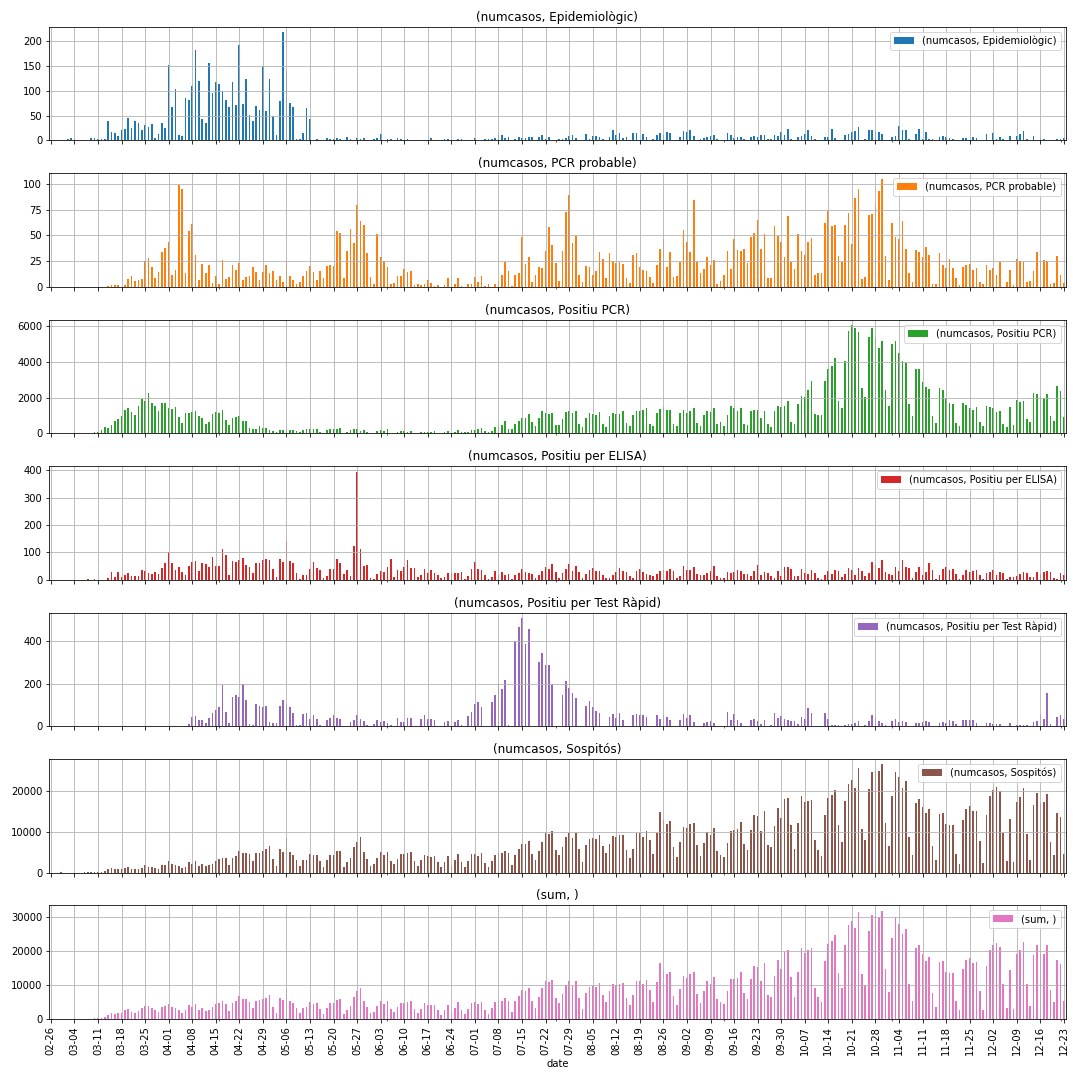
\includegraphics[width=\linewidth]{plotpermethod.png}
     \caption{Data set variables plot}
     \label{fig:Dataset_variables_plot}
 \end{figure}

In Figure \ref{fig:Dataset_variables_plot} is shown a plot that displays the amount of data that represents the total infected people separated by the type of case: "Epidemiològic", "PCR probable", "Positiu PCR", "Positiu per ELISA", "Positiu per test ràpid" and "Sospitós". Since the data of "Sospitós" type represents the majority of the data contained in the sum of all types and its status has not been confirmed yet, we have decided to filter all the cases that are part of this category.

Since there is not a huge amount of data until the moment, a data augmentation function have been implemented in order to see how this variation of data affects to the performance of each of the algorithms studied.

\subsection{Data Preprocessing}
Our dataset, as mentioned previously, is build using 2 data sets found in the Catalonia open-source web-page.

For the first dataset the information about infected people are extracted, while in the second one the death people statistics are obtained. For both data sets the same pre-processing steps have been applied.

In the first step we have dealt with missing values and due to the fact we are working with almost all the fields present in the data set and their frequency was really low, it has been decided to remove them from the data set. Also, all the missing values were in the region field and since we needed this information to compute the histogram, it made no sense to replace the missing values with the mean of the regions or other kind of metric since we think that this would lead to obtain less accurate results.

In the second step, both data sets have been grouped by date. Then, for the infected people dataset the cases where the type of case was "Suspicious" and not "Positive PCR" have been filtered and only those with a positive result in their PCR have been used to compute the total number of infected people for each date group. Regarding the death data set, once removed the missing values the total amount of death people for each date has been computed. For the missing values once computed the amount of infected and death people and joined both columns, 0 values have been fixed.

The next step is to compute the region's histogram for each of the data set, which will be computed with the same methodology. To do so, the pivot table function of Pandas have been used. This function computes the sum of infected or death people, depending on the data set used, for each of the regions separated by date. For both histograms, the missing values will be replaced by 0 values. Once computed the histograms, the columns name will be changed adding the suffix '\_pos' or '\_death' in order to be able to differentiate each histogram. 

In the following step, the same process as for the region histogram computation have been followed to compute the histogram of infected and death people segregated by sex. In this case, a pivot table have also been created but using the sex description column, so the sum of infected or death people for each sex is obtained. The missing values has also been filled with 0's and the columns names have also been replace with a tag in order to differentiate them.

The last step aims to obtain the value of R0 for each date in the data set. This parameter is a growth coefficient that provides information about how many people will be infected because they have contact with an infected person. Ideally, we want this coefficient to be lower than 1, which indicated that the infections are decreasing. This parameter is computed as follows:
\begin{equation}
    \label{eqn:R0}
    R_0[i] = e^{\frac{\ln (\frac{P}{\frac {x[i-L]*P}{x[i-1]}-1})}{L-1}}
\end{equation}
where $i$ corresponds to the date for which we are computing this parameter, $L$ corresponds to the lookback, which is 7 in our case, and $P$ is the population of the region. In this case, the parameter $P$ is around 7,566 million habitants.

Finally, a vector containing the number of infected people, the amount of deaths, the region histogram and the sex histogram for both (infected and deaths) have been obtained for each date in the previous datasets.

\subsection{Data Augmentation}
Due to this disease was unknown before the outbreak in December 2019 in Wuhan, China, the data available for Catalonia comprises from 26th of February to the 31st of December 2020.

Since we want to study the performance of different machine learning models in the prediction of the COVID-19 evolution, it's desirable to work with more data than the available, for this reason data augmentation has been applied in our data set.

As mentioned previously our data contains information about the number of infected and death people, the region histogram of infected and death people and the number of males and females that were infected and the ones that were death. We have assumed that slight variations in this data would not affect the performance of our models since the difference with the actual data is not huge. For this reason, we have decided to apply Gaussian noise with a little variance in each sample of our dataset. 

In the next sections the results obtained applying this technique will be reviewed and discussed.

\section{Methods}

The purpose of this section is to provide a brief introduction to each of the architectures used in the scope of this project.

\subsection{Multi-Layer Perceptron}

Neural Networks architectures have proven to be good fits for classification and regression tasks. These are composed of layers of fully connected units or neurons that use an aggregation function and a non-linear activation function to produce a non-linear mapping. Given a sufficient amount of layers and neurons in the architecture, the capability to generalize and extract features from the data increases considerably.

    An MLP Regressor trains iteratively and computes the partial derivatives of the loss or cost function with respect to the model parameters (weights and biases) to update them and find the optimal values that are able to minimize the error.

    As it corresponds to one of the main topics seen in the Neural Computation subfield of the Computational Intelligence subject, it was a clear candidate model architecture for a regression task on the data. In order to "alleviate" the Curse of Dimensionality issue that has a strong impact in deep architecture models a data augmentation process is carried out as well.

\subsection{Support Vector Regression}

Support Vector Regression is similar to Linear Regression in that the equation of the line is y= wx+b In SVR, this straight line is referred to as hyperplane. The data points on either side of the hyperplane that are closest to the hyperplane are called Support Vectors which is used to plot the boundary line.
Support Vector Regressor gives us the flexibility to define how much error is acceptable in our model and will find an appropriate line (or hyperplane in higher dimensions) to fit the data.

In this document an hyper-parameter search in order to obtain which are the best values for them have been performed. In \cite{Smola04atutorial} a detailed tutorial covering the impact of each parameter is found. The following parameters have been tunned in our analysis:

\begin{itemize}
    \item C: Regularization parameter. The strength of the regularization is inversely proportional to C. Must be strictly positive.
    \item gamma: Kernel coefficient for ‘rbf’, ‘poly’ and ‘sigmoid’.
    \item kernel: A kernel helps us find a hyperplane in the higher dimensional space without increasing the computational cost. Usually, the computational cost will increase if the dimension of the data increases.
    \item degree: Degree of the polynomial kernel function (‘poly’). Ignored by all other kernels.
\end{itemize}

The values tested for each parameter have been defined using trial and error method in order to adjust and obtain the best ones.

\subsection{Adaboost}

Boosting is a general ensemble method that creates a strong classifier from a number of weak classifiers. This is done by building a model from the training data and then creating a second model that attempts to correct the errors from the first model. Models are added until the training set is predicted perfectly or a maximum number of models are added.
AdaBoost was the first really successful boosting algorithm developed for binary classification, introduced by \cite{10.1006/jcss.1997.1504}. It can be used to boost the performance of any machine learning algorithm. It is best used with weak learners, which are models that achieve accuracy just above random chance on a classification problem.
The most suited and therefore most common algorithm used with AdaBoost are decision trees with one level. Due to these trees are so short and only contain one decision for classification, they are often called decision stumps.
In this project an hyper-parameter analysis has also been performed for this algorithm. Different values for the learning rate have been tested and the number of estimators has been tunned.

\subsection{Random Forest Regression}

Random Forest Regressors (RFR) in an ensemble algorithm which extension used in our work was presented by \cite{10.1023/A:1010933404324}, that uses a combination of unpruned binary tree predictors such that each tree depends on the values of a random vector sampled independently and with the same distribution for all trees in the forest. The generalization error for forests converges almost surely to a limit as the number of trees in the forest becomes large. 

While in traditional or standard trees like CARTs, each node is split using the best split among all variables in the growing phase, in RF each node is split using the best among a subset of predictors randomly chosen at that node. This somewhat counter-intuitive strategy turns out to perform very well compared to many other classifiers, including discriminant analysis, support vector machines, and neural networks and is robust against noise and overfitting thanks to the random decision forests as they help correcting this decision trees' habit (injected randomness in forests aims to drecrease the variance). 

\begin{figure}[ht!]
   \center
   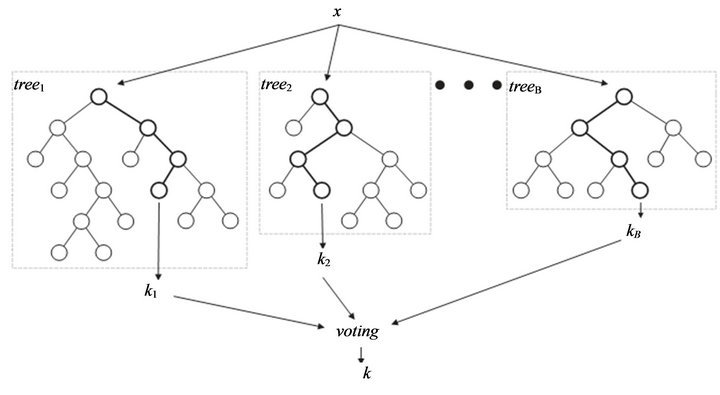
\includegraphics[width=\linewidth]{RF-architecture.jpeg}
   \caption{\label{fig:RF}Random Forest diagram}
\end{figure}

Figure \ref{fig:RF} portrays an schematic of an standard inference in RF, where the algorithm uses the inference output given by the various inner trees and a voting mechanism to produce a final prediction. In contrast, the implementation used in this work combines and produces a result by averaging the probabilistic prediction of the individual regressors.

Althought many parameters could be tunned such as the maximum depth of the trees or the minimum number of samples per split, we will concentrate in the most important ones: the number of trees in the forest and the number of variables per subset at each node.

With this in mind, we thought RFR would be a good fit to generate a baseline to be compared with other methods.

\subsection{LSTM}

Recurrent Neural Networks (RNN) are Artifical Neural Networks specially useful on predicting regression in data with a high temporal dependency. RNN are proven to be excellent at learning the time component of signals very efficiently thanks to the memory embedded into their architecture. These networks are characterized by having LSTM (Long Short Term Memory) and GRU (Gated Recurrent Units) layers in their architecture.

The LSTM algorithm was first proposed in 1997 by Hochreiter, Sepp and Schmidhuber \cite{hochreiter1997long} and has revolutionize the fields of handwriting recognition \cite{graves2008offline}, semantic parsing \cite{jia2016data}, robot control \cite{mayer2008system}, speech recognition \cite{graves2005framewise} and time series prediction \cite{schmidhuber2005evolino}. They also have been used in commercial products such as Google Voice, Google Translate, Apple's Siri, Amazon's Alexa.

\begin{figure}[!ht]
    \center
    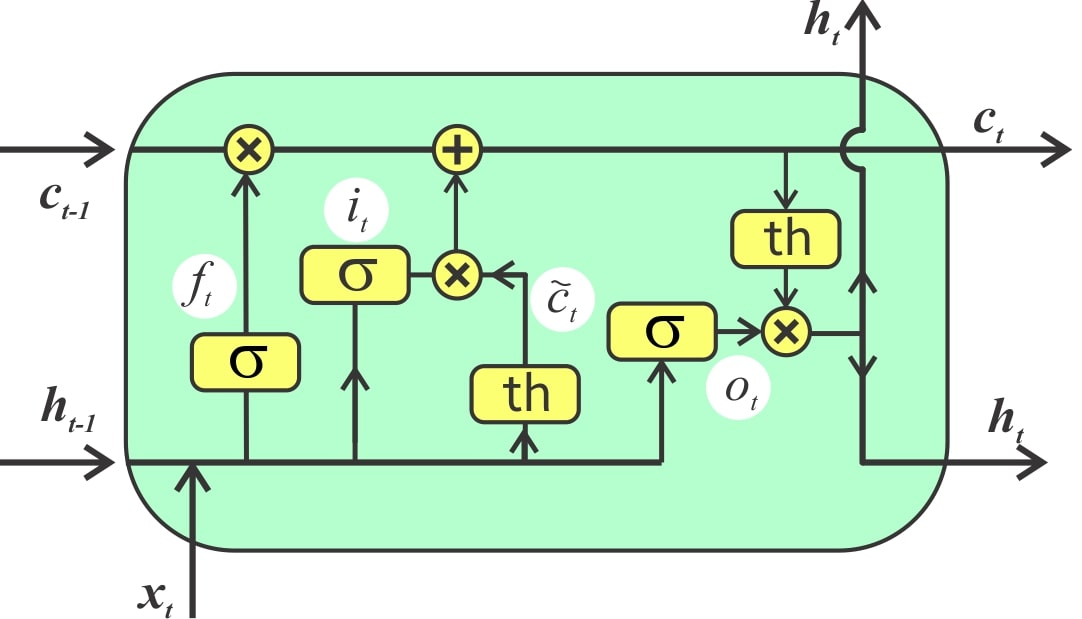
\includegraphics[width=\linewidth]{lstm-cell.jpg}
    \caption{\label{fig:LSTM-cell}LSTM cell diagram}
\end{figure}

The LSTM architecture is described in \ref{fig:LSTM-cell}\cite{LSTM} and follows different stages. The first step is the forget gate $f_t$ \ref{eqn:forget_gate} followed by the input gate $i_t$ \ref{eqn:input_gate}. The third stage is the cell state $C_t$ \ref{eqn:cell_state} then the output gate $o_t$ \ref{eqn:output_gate} and finally the final stage where the output is computed $h_t$ \ref{eqn:final_stage}.

\begin{equation}
    \label{eqn:forget_gate}
    f_t = \sigma(W_f \cdot [h_{t-1}, x_t] + b_f)
\end{equation}
\begin{equation}
    \label{eqn:input_gate}
    i_t = \sigma(W_i \cdot [h_{t-1}, x_t] + b_i)
\end{equation}
\begin{equation}
    \begin{split}
    \label{eqn:cell_state}
    \tilde{c_t} = tanh(W_C \cdot [h_{t-1}, x_t] + b_C) \\
    C_t = f_t \otimes C_{t-1} + i_t \otimes \tilde{c_t}
    \end{split}
\end{equation}
\begin{equation}
    \label{eqn:output_gate}
    o_t = \sigma(W_0 \cdot [h_{t-1}, x_t] + b_0)
\end{equation}
\begin{equation}
    \label{eqn:final_stage}
    h_t = o_t \otimes tanh(C_t)
\end{equation}

Where $x_t$ denotes the input vector. $h_{t-1}$ is the output of the previous LSTM cell. $b_*$ denotes the bias layer of the * gate. $W_*$ is the weight matrix for the * layer.

Because of the good performance of these architectures in the prediction of time series, we thought it would be a good fit for the task in hand.

\subsection{BLSTM}

Unlike Unidirectional LSTM only preserves information of the past because the only inputs it has seen are from the past, bidirectional lstm \ref{fig:BLSTM} or (BLSTM) stores information from the past and future inputs. This approach from unidirectional is that with an LSTM that also runs backwards you preserve information from the future and using the two hidden states combined you are able in any point in time to preserve information from both past and future.

\begin{figure}[!ht]
    \center
    \includegraphics[width=\linewidth]{BLSTM.png}
    \caption{\label{fig:BLSTM}BLSTM diagram}
\end{figure}

What they are suited for is a very complicated question but BLSTMs show very good results as they can understand context better. For this reason, it was integrated also in the models to give it more capabilities on capturing the context of the data.

As the COVID-19 data has a high context dependency, the bidirectionality of the network could really help the network to more accurately predict the patterns in the data.

\subsection{Hyperparameter and Model Selection}

In order to choose the set of optimal parameters of the learning process for each algorithm, we have used different techniques depending on the algorithm specificities. In the case of the traditional ML Regressors, and considering the dimensions of our initial data set, we considered an exhaustive search over a predefined range of specific parameter values the best suit. This was performed guided by a \textit{Mean Squared Error} metric and measured by a 10-fold cross-validation on the data set.

    Concerning the neural models, a manual search of hyperparameters was performed given the high computational cost that an exhaustive search would have required. Nonetheless, as the amount of data available for this task (even after a data augmentation process) was not as extended as it can be in usual deep learning tasks, we decided to carry out a 10-fold cross-validation for the neural models as well.

\section{Experiments}

This section aims to provide a clear description of the different experiments and methods carried out in the scope of this project. A baseline of traditional ML Regressors was performed as an initial approach to be compared with following neural experiments such as the temporal modeling with an RNN regressor.

\subsection{Baseline of traditional Machine Learning Regressors}

This experiment consists in our first approaches resulted by our initial ideas on how to pin down the problem by fitting the data set using traditional regression methods. This would also serve as a qualitative look on the data additional to the statistical analysis and provide baseline metrics to be compared with advanced neural models. The aforementioned explained models: MLP, SVR, Adaboost, and RFR compose the different set of architectures used in this experiment, which are all evaluated using the same methodology: performing an exhaustive hyper-parameter search for the most relevant selected architecture-specific parameters, averaging over a 10-fold cross-validation and using a MSE as an error metric. In order to provide more data and avoid overfitting, a data augmentation process is carried out by adding different noise variances.

The concrete hyper-parameters tested for each one of the architectures are the following:

\begin{itemize}
    \item MLP: Different parameters tested include: the number of hidden layers and units per layers, where combinations of 5, 8, 10, 30 and 50 units were checked within one or two at most hidden layers; ReLU or hyperbolic tan function as activation functions; Stochastic Gradient Descent or Adam as weight optimization techniques; constant, inverse scaling to a power of .5, .3 or .1 and adaptive learning rates and a momentum of .9
    \item SVR: The parameters we wanted to focus on this algorithm were the ones related to the kernel used to treat the data as if it had a higher dimension, such as Radial Base Function, linear or polynomial kernels and the C regularization parameter, used to assign a penalization degree to the slack variables, where low values between 1.0 and 10.0 were chosen to leave space for some mislabelings.
    \item Adaboost: We focused on the parameters considered more important in an Adaboost Regressor such as the number of boosted ensemble estimators and their contribution provided by a learning rate. 150, 200 and 500 estimators were tested along learning rates of 1.0, .9, .8 and .5
    \item RFR: The same criteria as Adaboost was followed given their categorization as ensemble learners were the most important parameters were tested, which in this case is the number of inner trees. Again, 150, 200 and 500 estimators define the tested range.
\end{itemize}

\subsection{Temporal modeling with RNN regressor}

The goal of this experiment was to validate an RNN architecture for fitting the available data on this project. Four different architectures are proposed. The models will be evaluated following the same methodology as in the previous experiment, a 10-fold cross validation for all the data, augmenting the data by adding 2 different noise variances, and with $MSE$, $max_{error}$ and $r^2$ correlation as validation metrics.

Before the definition of the architectures, a rearrangement of the data must be done. Unlike the previous models, RNN networks have a temporal dependency to learn and require the input tensors to have multiple consecutive instances of the training set instead of only one sample. In order to do that, a rearrangement of the data was performed where for each sample in the training set, lookback ($lb$)-1 instances are concatenated in order to obtain a tensor of shape $(lookback, n_{features})$ for each training sample of the network. With this, we transformed the $(n_{instances}, n_{features})$ data set used in the previous experiment to a $(n_{instances}, lb, n_{features})$ datset suitable for these networks. 

\begin{figure}[!ht]
    \center
    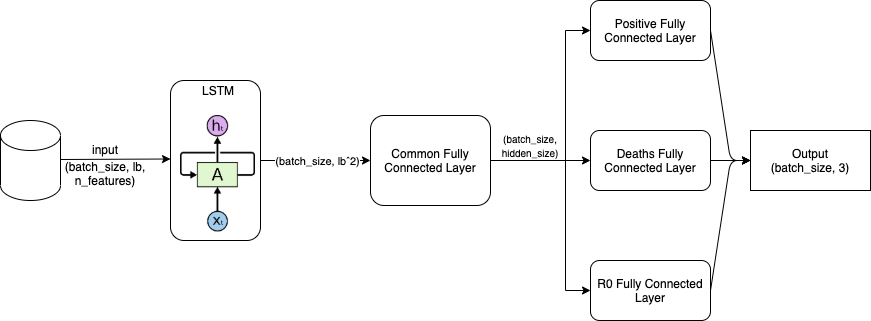
\includegraphics[width=\linewidth]{Networks-LSTM-Hidden}
    \caption{\label{fig:LSTM-hidden}LSTM network with common fully connected layer}
\end{figure}

The first architecture \ref{fig:LSTM-hidden} consists on an LSTM layer followed by a fully connected layer and three fully connected output layers, one for each value to be predicted (positive cases, deaths and $R_0$). The objective of this architecture is to be a compromise between having a network for each parameter to be predicted and a network that predicted the 3 values while sharing all the weights and parameters between them. With this architecture, we allow the network to learn the particularities of each predicted value while also learn the patterns that apply to all 3 output values with the common fully connected layer.

\begin{figure}[!ht]
    \center
    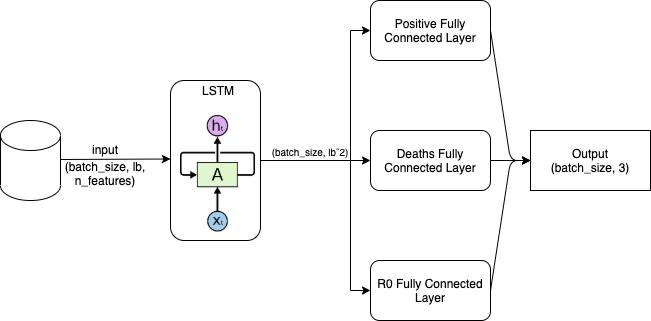
\includegraphics[width=\linewidth]{Networks-LSTM-NoHidden}
    \caption{\label{fig:LSTM-nohidden}LSTM network with no common fully connected layer}
\end{figure}

The second architecture \ref{fig:LSTM-nohidden} is a modified version on the first one. The LSTM output is directly connected to the individual fully connected layers for the output values. With this suppression of the common fully connected we expected the network to more easily learn each output independently. The motivation for this change was an observation of a trade-off between the improvement of an output value and the decrease in accuracy in other outputs.

\begin{figure}[!ht]
    \center
    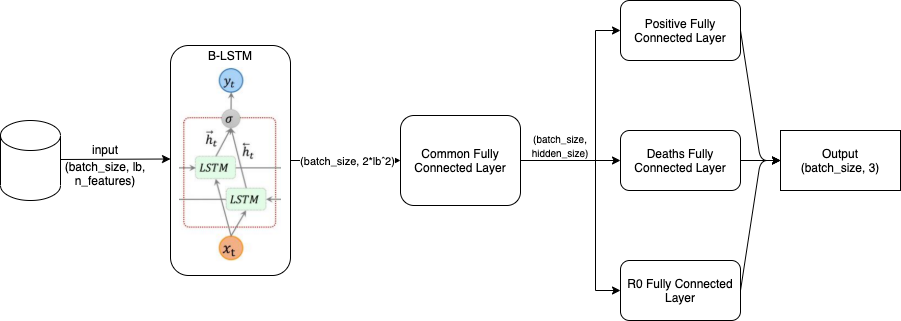
\includegraphics[width=\linewidth]{Networks-BLSTM-Hidden}
    \caption{\label{fig:BLSTM-hidden}B-LSTM network with common fully connected}
\end{figure}

\begin{figure}[!ht]
    \center
    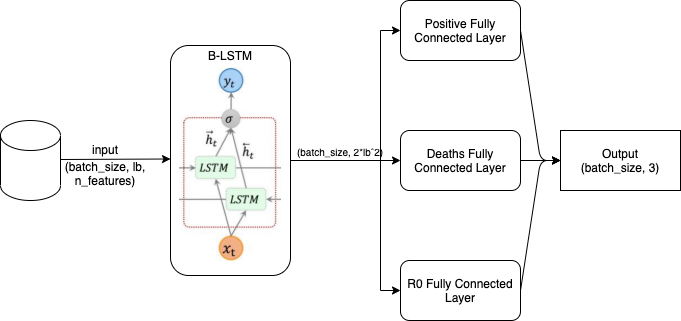
\includegraphics[width=\linewidth]{Networks-BLSTM-NoHidden}
    \caption{\label{fig:BLSTM-nohidden}B-LSTM network with no common fully connected layer}
\end{figure}

The third \ref{fig:BLSTM-hidden} and the fourth \ref{fig:BLSTM-nohidden} architectures were the first and the second RNNs but with the LSTM layer replaced by a B-LSTM layer to better adapt to the dependencies between the data of the different days.

The number of units for both BLSTM and LSTM layers were tested for 8, 16, 32, 64 and 128. In the network configurations that apply, 50, 100 and 200 units for the common fully connected layer were tried. These values were chosen because of the best configurations that were obtained for the MLP regressor. The models were all trained using an Adam optimizer with an Exponential decay learning rate as the first epochs on the training process make the most change to the model's learning. Exponential Decay also helps to outweight the impact of the noise added in the data augmentation stage of the pre-processing, as noise in the data can worsen the stability of the loss function's minimum finding process. 

Each of the three outputs were evaluated separately with their own loss function (MSE in all cases) in order for each dedicated final layer to only be updated with the gradients of their output. The gradients are then added in the previous layers to be backpropagated to the rest of the network.

Finally the experiment with all these parameters were performed with the data restructured with a lookback value of 8 and a 10-fold cross validation. The SARS-Cov-2 disease has an estimateed incubation time of two weeks, because $R_{0}$ already provides the network with some context on the tendency of the values on the previous 7 days are, makes sense to set the lookback value to 8 to provide the network with 15 days of context to make an informed prediction.

All models were tested using the 92 features for each training day described previously: the positive cases, the deaths, the location histogram for positive cases, the location histogram for deaths, the sex distribution for positive cases, the sex distribution for deaths and the $R_0$ value for that day. During the cross validation procedure, the initial weights for the 0th fold are stored and then set in all other folds so that the network is initialized the same way in all folds and a random seed is set for better reproducibility of the results. The best results were found to have 64 LSTM/B-LSTM units and 100 hidden units for the first and third models.

As a last test for the architecture was performed with the same 3 variables to be predicted as input with the objective of consecutively predict the values for the day $t$ and update the input with them to predict the day $t+1$ and so on. With this test we were able to make a prediction for the positive cases, the deaths and the $R_0$ values for the next 90 days.


\section{Results and Discussion}

The results achieved on the previously explained experiments produced the results present in \ref{tab:Results}. For all the models in the first experiment, a 10-fold cross validation was used to determine the best parameters in for them. After the models were trained a full inference was performed on all the data, as seen in \ref{fig:allpredictions}.The best model was obtained with an RFR architecture with 200 estimators. This model performed better in all metrics except for the $R_0$'s max error metric. However, Adaboost presented a marginal improvement over the results on RFR. 

\begin{figure}[!ht]
    \center
    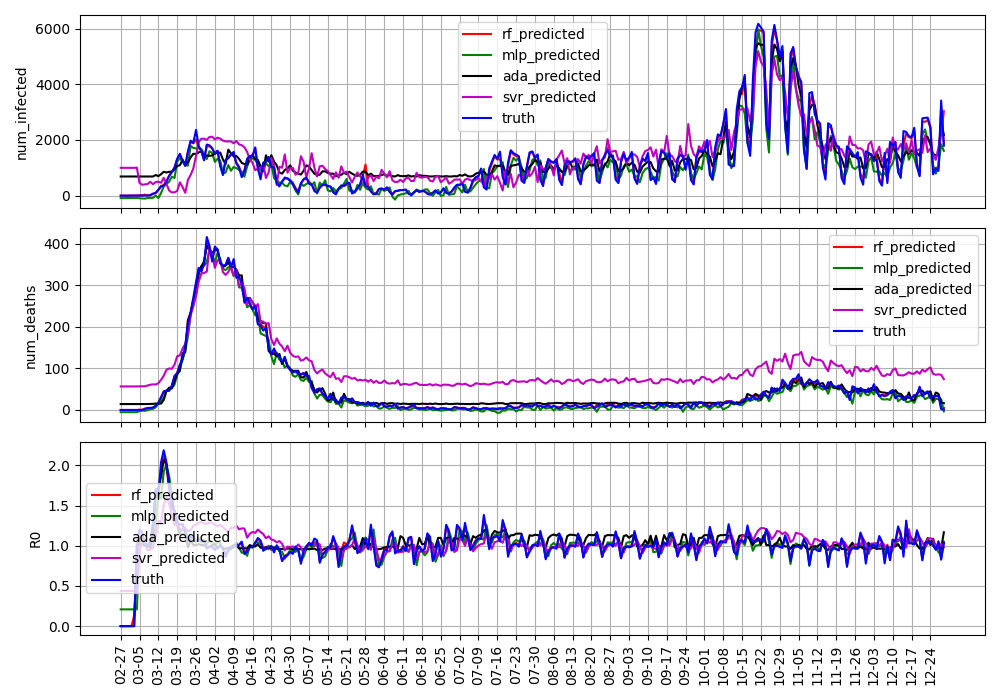
\includegraphics[width=\linewidth]{allpredictions}
    \caption{\label{fig:allpredictions}Inference on all data set for the 10th fold model}
\end{figure}

The Random Forest architecture creates multiple decision trees with some features assigned to them and then it performs an aggregation on all the outputs of the branches. This makes the algorithm way more robust to overfitting and it seems to be the case. However, even if the algorithm was able to discriminate better the different regions of data points in the training data much better than the other 3 methods, because of the underlying structure of the algorithm, RFR can't easily extrapolate patterns from a time series prediction data set. 

Because of that uncertainty in the generalization capabilities of the RFR method, we explored some Deep Learning Time Series prediction methods as described in the second experiment. In the same table \ref{tab:Results}, the results for all 4 networks are compared to the results obtained with the RFR architecture. They all delivered very promising results, achieving at least half of the error in $MSE$ and increasing the correlation coefficient as well as significantly decreasing the $Max_{error}$. Even if all the models performed well, the best results for this experiment were achieved by the fourth model. This model consisted on a BLSTM implementation without a common hidden layer. 

The best model achieved an $MSE$ of 0.00002 for the positive cases, 0.000015 for the deaths and an error of 0.000147 for the $R_0$ value. It also accomplished $r^2$ values of 0.998, 0.999 and 0.943 for positive, deaths and $R_0$ respectively. Finally the model achieved $Max_{error}$ values of 0.014, 0.01 and 0.054 for the output values.

\begin{table*}[t!]
 \centering
 \resizebox{\textwidth}{!}{
     \begin{tabular}{|c|c|c|c|c|c|}
     \multicolumn{1}{c}{Architecture} & features & Output   & \multicolumn{1}{c}{mse} & \multicolumn{1}{c}{r2} & \multicolumn{1}{c}{max\_error} \\
     \hline \hline
     BLSTM No Hidden                  & 92       & positive & 0.000020                & 0.997892               & 0.014067                       \\
     BLSTM No Hidden                  & 92       & deaths   & 0.000015                & 0.998707               & 0.010581                       \\
     BLSTM No Hidden                  & 92       & r0       & 0.000147                & 0.942740               & 0.053851                       \\
     \hline
     BLSTM No Hidden                  & 3        & positive & 0.000195                & 0.974363               & 0.044300                       \\
     BLSTM No Hidden                  & 3        & deaths   & 0.000066                & 0.994793               & 0.022734                       \\
     BLSTM No Hidden                  & 3        & r0       & 0.000198                & 0.924468               & 0.069665                      \\
     \hline
     \end{tabular}
 }
 \caption{\label{tab:3featsResults}Metrics for the best model and the 3 features reduced model}
 \end{table*}

The model was finally inferred for all the data set and the three output values are shown in \ref{fig:alldatainference}. From this graph we can see that the model is able to learn the valley pattern that occurs weekly in the positive cases array. 

 \begin{figure}[!ht]
     \center
     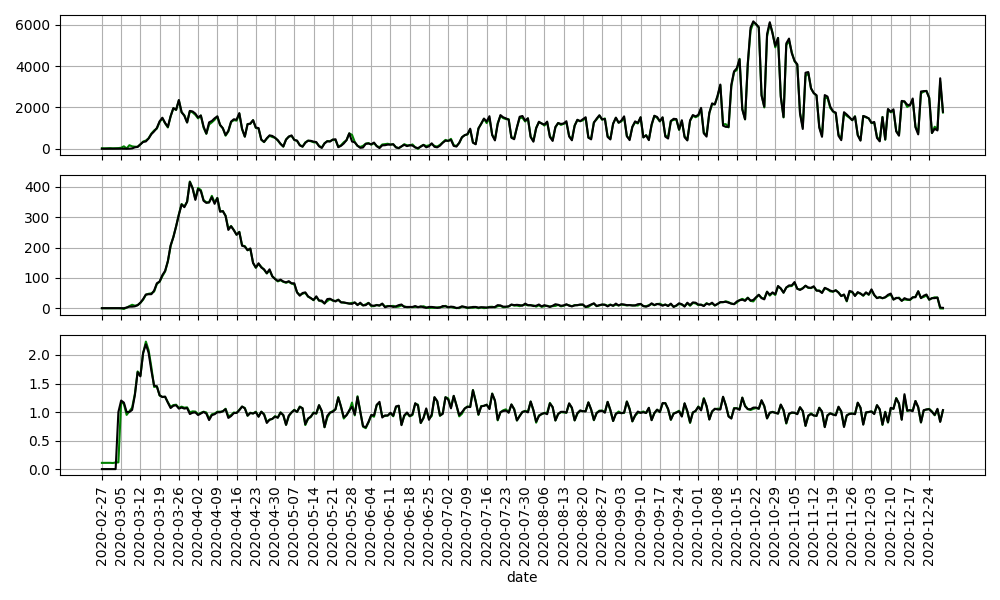
\includegraphics[width=\linewidth]{blstm-alldata}
     \caption{\label{fig:alldatainference}Inference of all data set in the 10th fold trained model}
 \end{figure}

A third experiment was performed, extending the RNN experiment that yielded the best model. In this experiment, the goal was to make a model capable of recursively predict the day $t+1$ from the day $t$ as has been explained in the previous section. With this model, we were able to cast a prediction on multiple days ahead of the last day on our data set without having a big loss in accuracy as shown in the results table \ref{tab:3featsResults}. We performed a 90 day forecast on the model and obtained the predictions shown in \ref{fig:90daypred}.

From the predictions we can see that the model foresees a rise and a spike in positive cases in January and February, which is very much what we would expect given that the latest evidence that the model has is that the positive cases are increasing at a similar rate than in October. It also predicts that the $R_0$ value and the deaths values will follow similar trends to those in October-December as well.

 \begin{figure}[!ht]
     \center
     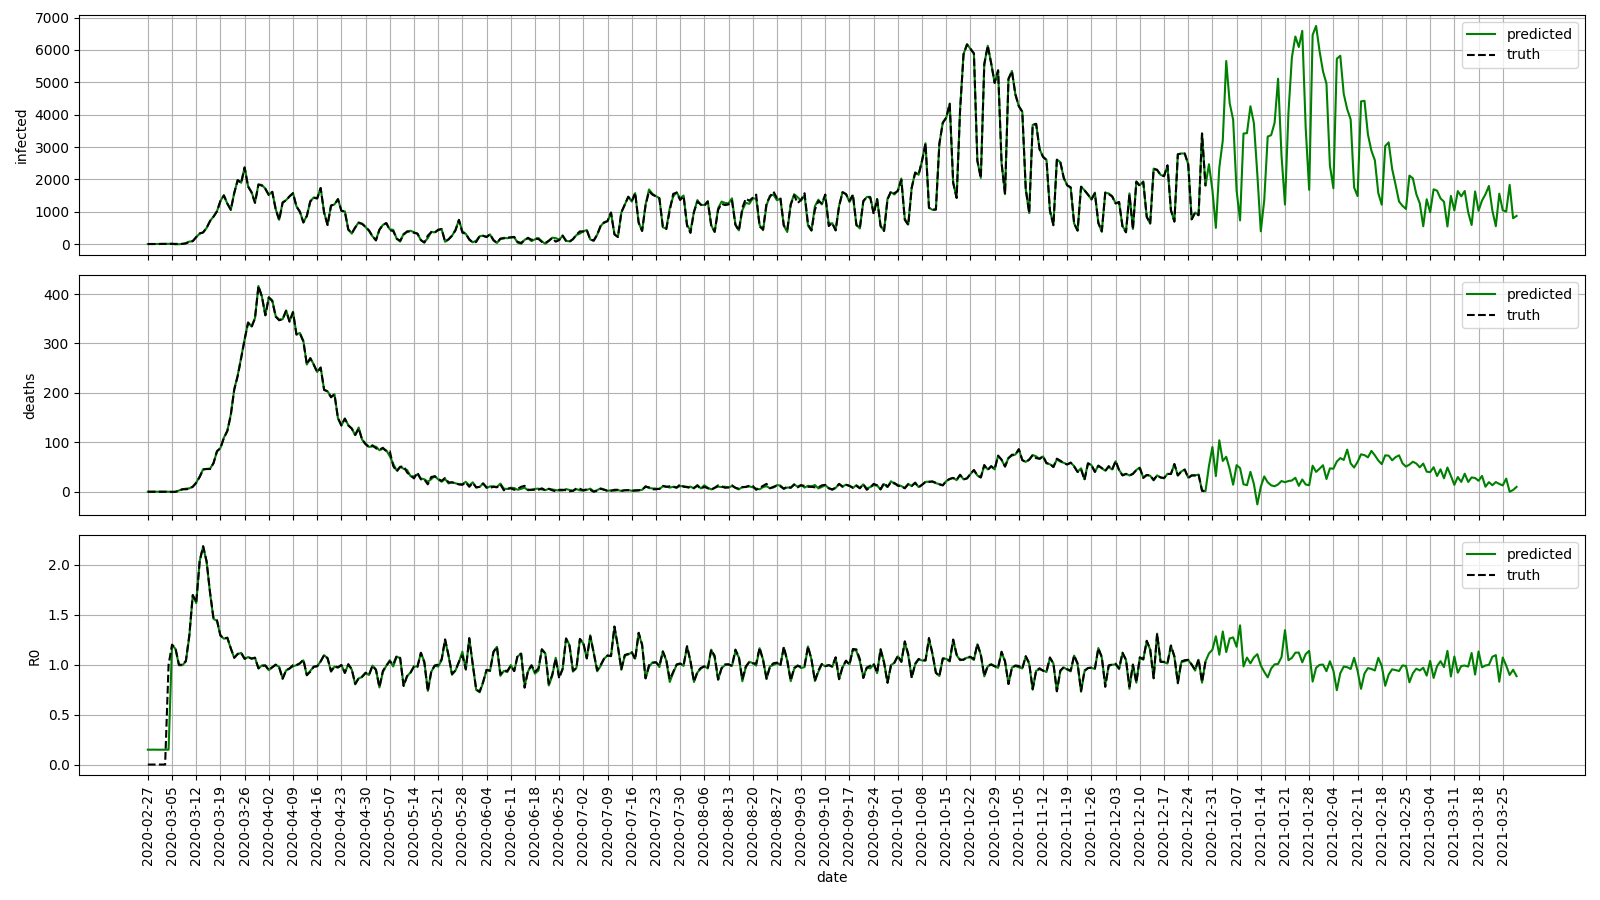
\includegraphics[width=\linewidth]{blstm3feats-90extension}
     \caption{\label{fig:90daypred}90 Day forecast using 3feature BLSTM Network}
 \end{figure}

Additionally a 900 day forecast was tried \ref{fig:900daypred}. However, the model failed to predict something reasonable because of two main factors. The error in the model's predictions is accumulated as each ouput is used for predicting the next day. The network has not learned to deal with negative numbers, as it is a variable that is not present in the real world and should not happen.

 \begin{figure}[!ht]
     \center
     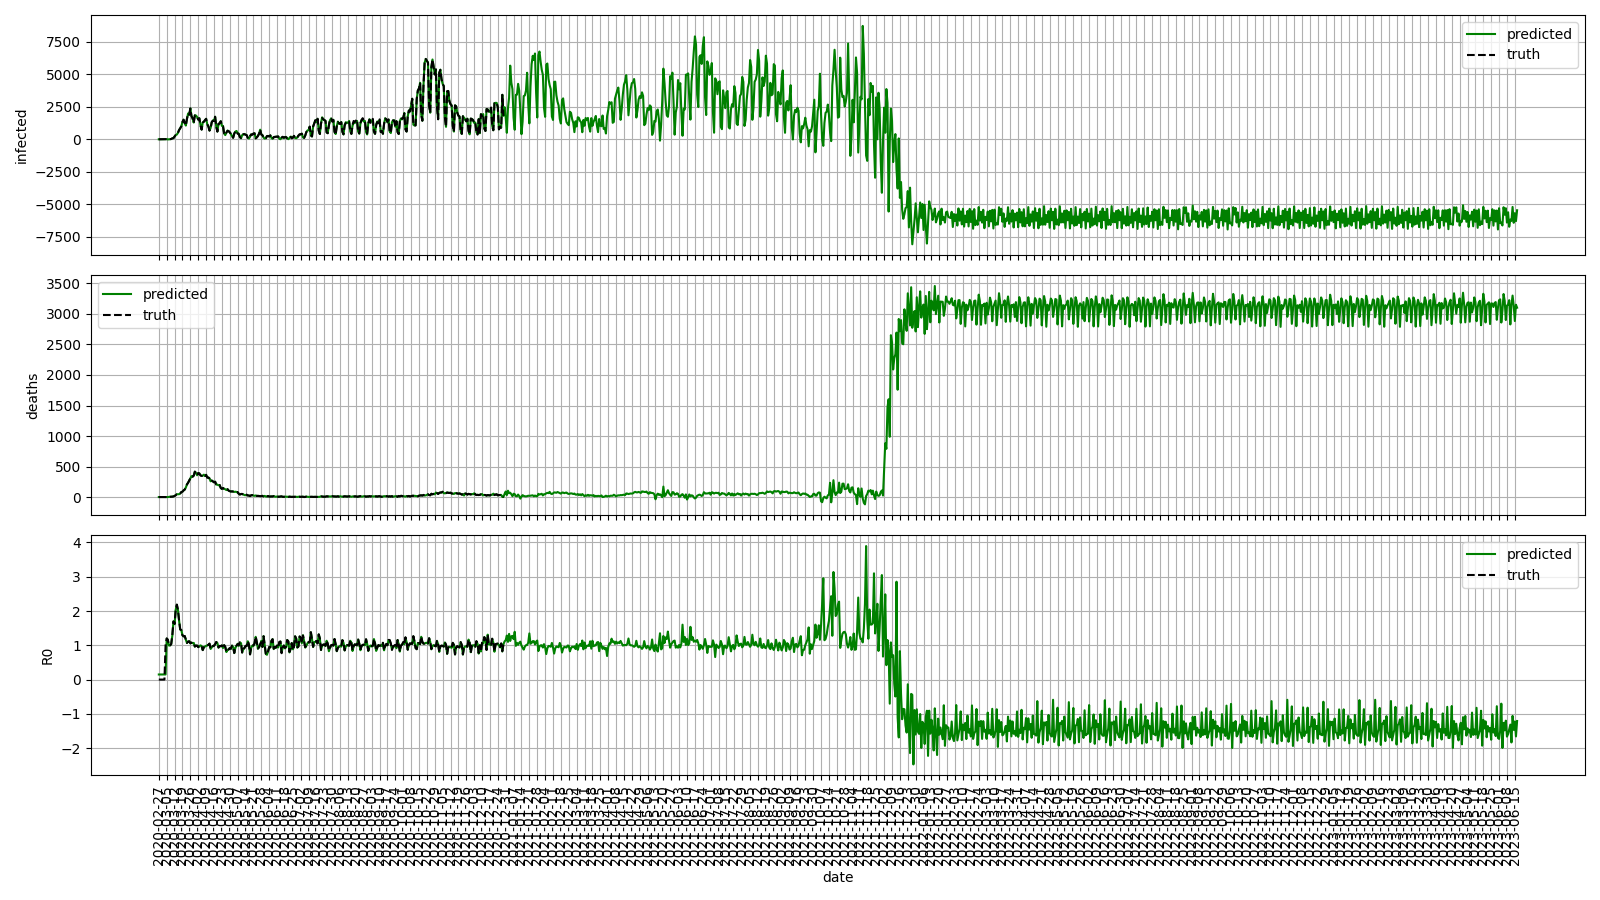
\includegraphics[width=\linewidth]{blstm3feats-900extension}
     \caption{\label{fig:900daypred}900 Day forecast using 3feature BLSTM Network}
 \end{figure}

 \begin{table*}[t!]
 \centering
 \resizebox{\textwidth}{!}{
     \begin{tabular}{|c|c|c|c|c|c|}
     Architecture    & Output   & Parameters                                                         & \multicolumn{1}{c}{MSE} & \multicolumn{1}{c}{$r^2$} & \multicolumn{1}{c}{Max Error} \\
     \hline \hline
     RFR              & positive & \{'n\_estimators': 200\}                                           & 0.000283                & 0.964868                                 & 0.062833                      \\
    RFR              & deaths   & \{'n\_estimators': 200\}                                           & 0.000035                & 0.996806                                 & 0.024604                      \\
    RFR              & $R_0$     & \{'n\_estimators': 200\}                                           & 0.000250                & 0.886291                                 & 0.080736                      \\
    \hline
    MLP             & positive & \{'hidden\_layer\_sizes': (50, 50), 'learning\_rate': 'constant'\} & 0.001033                & 0.849651                                 & 0.097124                      \\
    MLP             & deaths   & \{'hidden\_layer\_sizes': (50, 50), 'learning\_rate': 'constant'\} & 0.000163                & 0.985615                                 & 0.049893                      \\
    MLP             & $R_0$     & \{'hidden\_layer\_sizes': (50, 50), 'learning\_rate': 'constant'\} & 0.000748                & 0.599288                                 & 0.108641                      \\
    \hline
    SVR             & positive & \{'C': 4.0, 'degree': 1, 'gamma': 'scale', 'kernel': 'rbf'\}       & 0.003231                & 0.369218                                 & 0.103842                      \\
    SVR             & deaths   & \{'C': 1.0, 'degree': 1, 'gamma': 'scale', 'kernel': 'linear'\}    & 0.004272                & 0.347436                                 & 0.097379                      \\
    SVR             & $R_0$     & \{'C': 6.0, 'degree': 1, 'gamma': 'auto', 'kernel': 'rbf'\}        & 0.001525                & -0.613484                                & 0.136571                      \\
    \hline
    Adaboost        & positive & \{'learning\_rate': 1, 'n\_estimators': 150\}                      & 0.001536                & 0.693514                                 & 0.069253                      \\
    Adaboost        & deaths   & \{'learning\_rate': 0.5, 'n\_estimators': 150\}                    & 0.000138                & 0.986623                                 & 0.029070                      \\
    Adaboost        & $R_0$     & \{'learning\_rate': 1, 'n\_estimators': 200\}                      & 0.000616                & 0.655629                                 & 0.074724                      \\
    \hline
    LSTM            & positive & \{LSTM: 64, EmbeddingSize: 100, look\_back: 8\}                    & 0.000031                & 0.996484                                 & 0.014770                      \\
    LSTM            & deaths   & \{LSTM: 64, EmbeddingSize: 100, look\_back: 8\}                    & 0.000018                & 0.998263                                 & 0.012360                      \\
    LSTM            & $R_0$     & \{LSTM: 64, EmbeddingSize: 100, look\_back: 8\}                    & 0.000137                & 0.947085                                 & 0.053583                      \\
    \hline
    LSTM no hidden  & positive & \{LSTM: 64, look\_back: 8\}                                        & 0.000025                & 0.997250                                 & 0.012657                      \\
    LSTM no hidden  & deaths   & \{LSTM: 64, look\_back: 8\}                                        & 0.000020                & 0.998101                                 & 0.012931                      \\
    LSTM no hidden  & $R_0$     & \{LSTM: 64, look\_back: 8\}                                        & 0.000134                & 0.938387                                 & 0.042689                      \\
    \hline
    BLSTM           & positive & \{LSTM: 64, EmbeddingSize: 100, look\_back: 8\}                    & 0.000034                & 0.996252                                 & 0.017672                      \\
    BLSTM           & deaths   & \{LSTM: 64, EmbeddingSize: 100, look\_back: 8\}                    & 0.000017                & 0.998460                                 & 0.012038                      \\
    BLSTM           & $R_0$     & \{LSTM: 64, EmbeddingSize: 100, look\_back: 8\}                    & 0.000137                & 0.946801                                 & 0.047911                      \\
    \hline
    BLSTM no hidden & positive & \{LSTM: 64, look\_back: 8\}                                        & 0.000020                & 0.997892                                 & 0.014067                      \\
    BLSTM no hidden & deaths   & \{LSTM: 64, look\_back: 8\}                                        & 0.000015                & 0.998707                                 & 0.010581                      \\
    BLSTM no hidden & $R_0$    & \{LSTM: 64, look\_back: 8\}                                        & 0.000147                & 0.942740                                 & 0.053851 \\ \hline
    \end{tabular}
}
\caption{\label{tab:Results}Best parameters and metrics for all architectures tested}
\end{table*}

\section{Conclusions and future work}
\color{black}

The aim of this project was to be able to predict through the use of different ML models and available data in Catalonia open-source web-page the evolution of the COVID-19 disease.

Although traditional regression algorithms experimented in this study are able to provide a considerable performance, they are not able to match the capabilities of neural models that introduce temporal constraints, as it can be seen that the best results were obtained using Bi-LSTM without common hidden layers. This configuration lead us to obtain very good results with a low error in the metrics used. From these results we infer that adding a temporal context along with the input data is an interesting approach to be further explored.

To further check the generalization capability of our best model, we generated a future prediction for the upcoming 90 and 900 days of the evolution of the epidemic. It could be argued how the model provides reasonable inferences for short-term windows while fails if required to do so for longer window contexts. If we did the exercise of comparing the outputs from the model to the evolution about to come, we would probably observe huge discrepancies, due to the fact that the model does not contain the temporal and seasonality information.

On one hand, through the experiments performed we have seen that we are accurately able to predict the trend on the data that is now available with a high accuracy. We are also able to predict multiple days in advance even if the error accumulates.

On the other hand, we are aware that the available data was maybe too small, which sometimes limitates the techniques applied to this data in order to obtain good results.

As future work, in order to further improve the future predictions of our model, it would be necessary to include extra annotations the the existing data set concerning spatial and temporal features. For example, it would be necessary to include additional features as the environment ones, mobility index rates, restrictions imposed by the local authorities, vaccination rates or seasonality among others. Some of them, like the local restrictions contain such variability and imprecision that they could probably be treated as linguistic variables in a fuzzy system approach. 

\newpage

\bibliographystyle{abbrv}
\bibliography{Covid19Cat}

\newpage

\appendix

\listoffigures

\listoftables

\newpage

\section{Model MSE Losses}

\begin{figure}[H]
    \center
    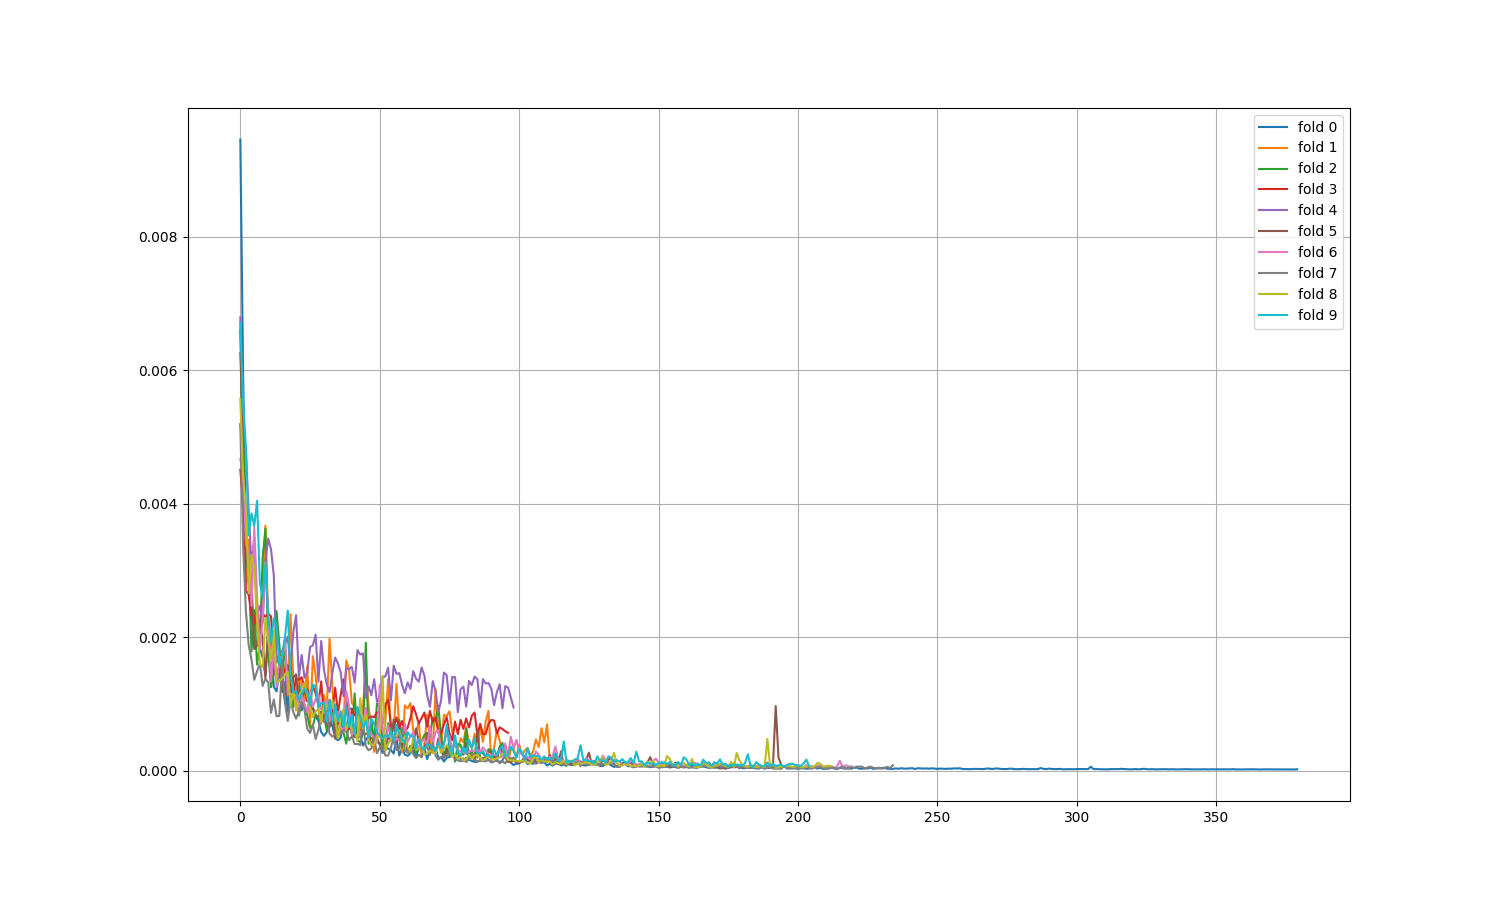
\includegraphics[width=\linewidth]{lstm-loss}
    \caption{validation loss function per fold in LSTM with no hidden layers model}
\end{figure}

\begin{figure}[H]
    \center
    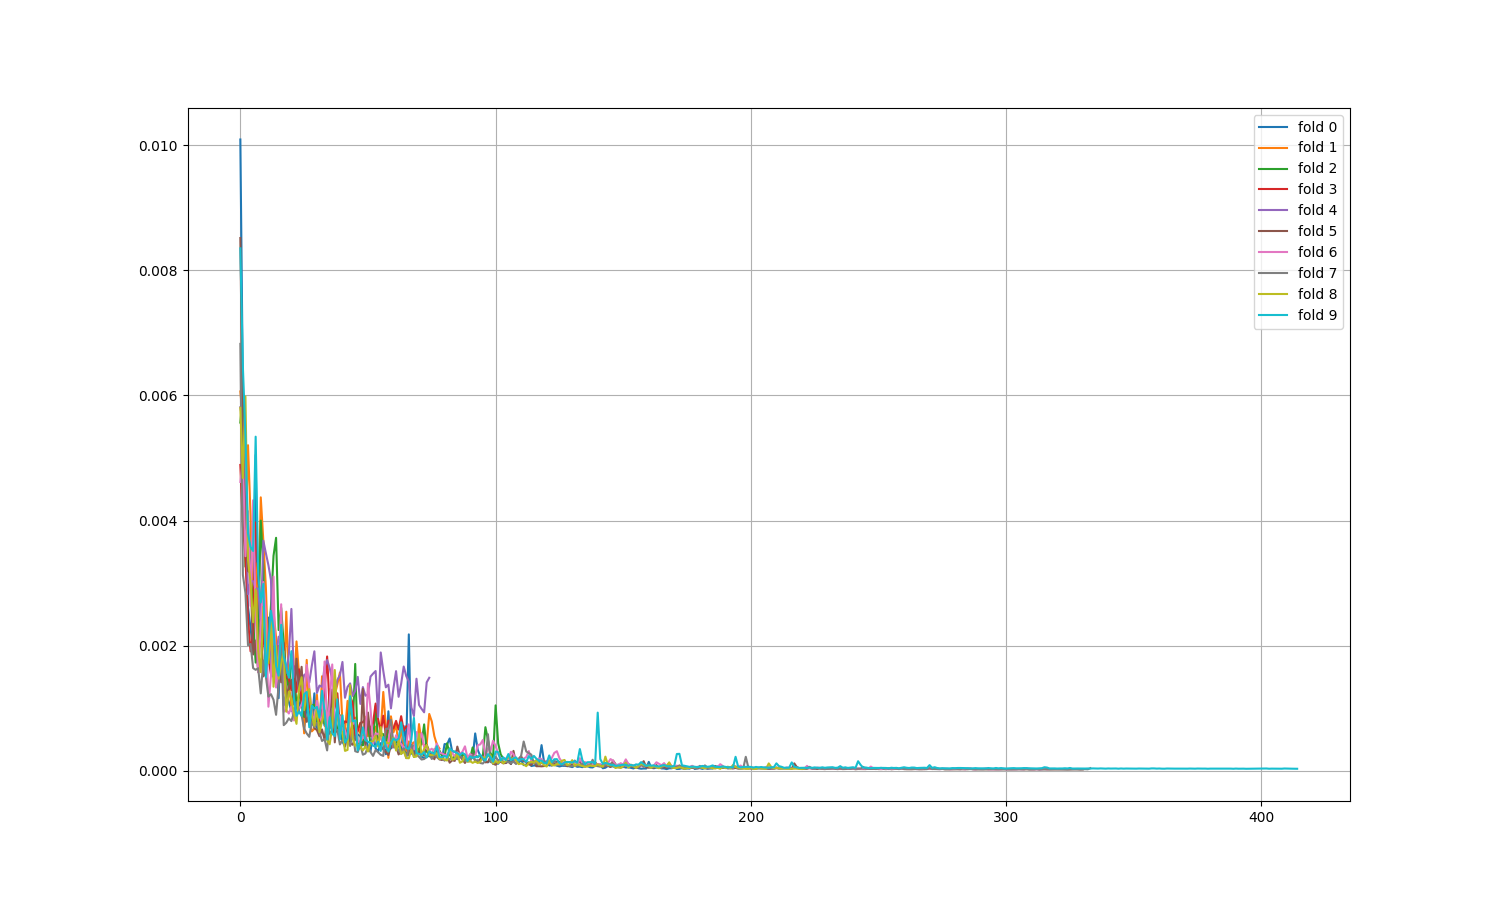
\includegraphics[width=\linewidth]{lstm-hidden-loss}
    \caption{validation loss function per fold in LSTM with hidden layer model}
\end{figure}

\begin{figure}[H]
    \center
    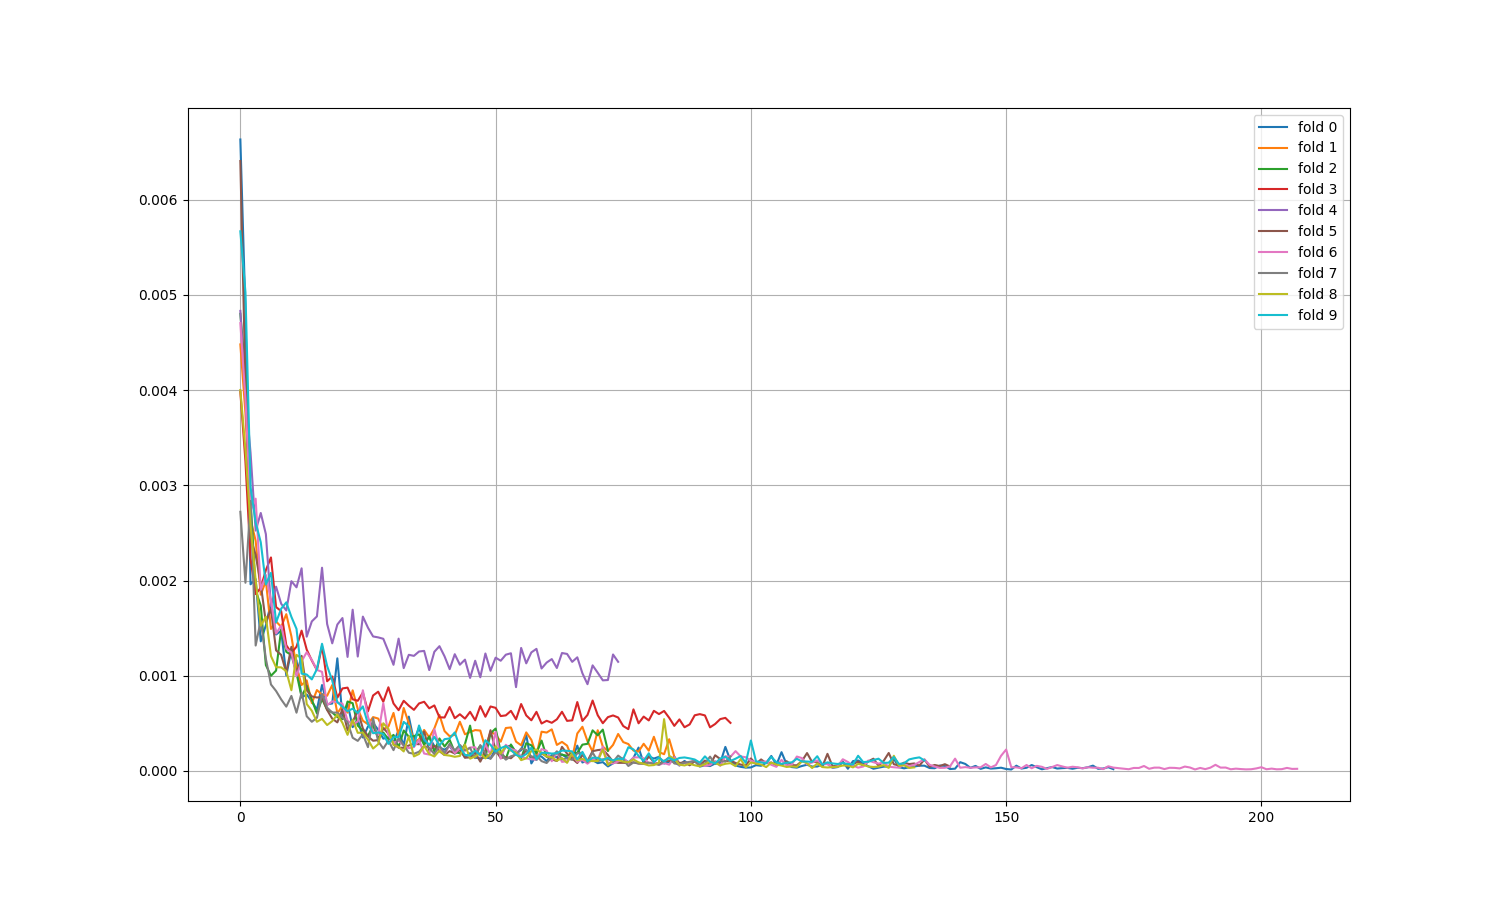
\includegraphics[width=\linewidth]{blstm-loss}
    \caption{validation loss function per fold in BLSTM with no hidden layers model}
\end{figure}

\begin{figure}[H]
    \center
    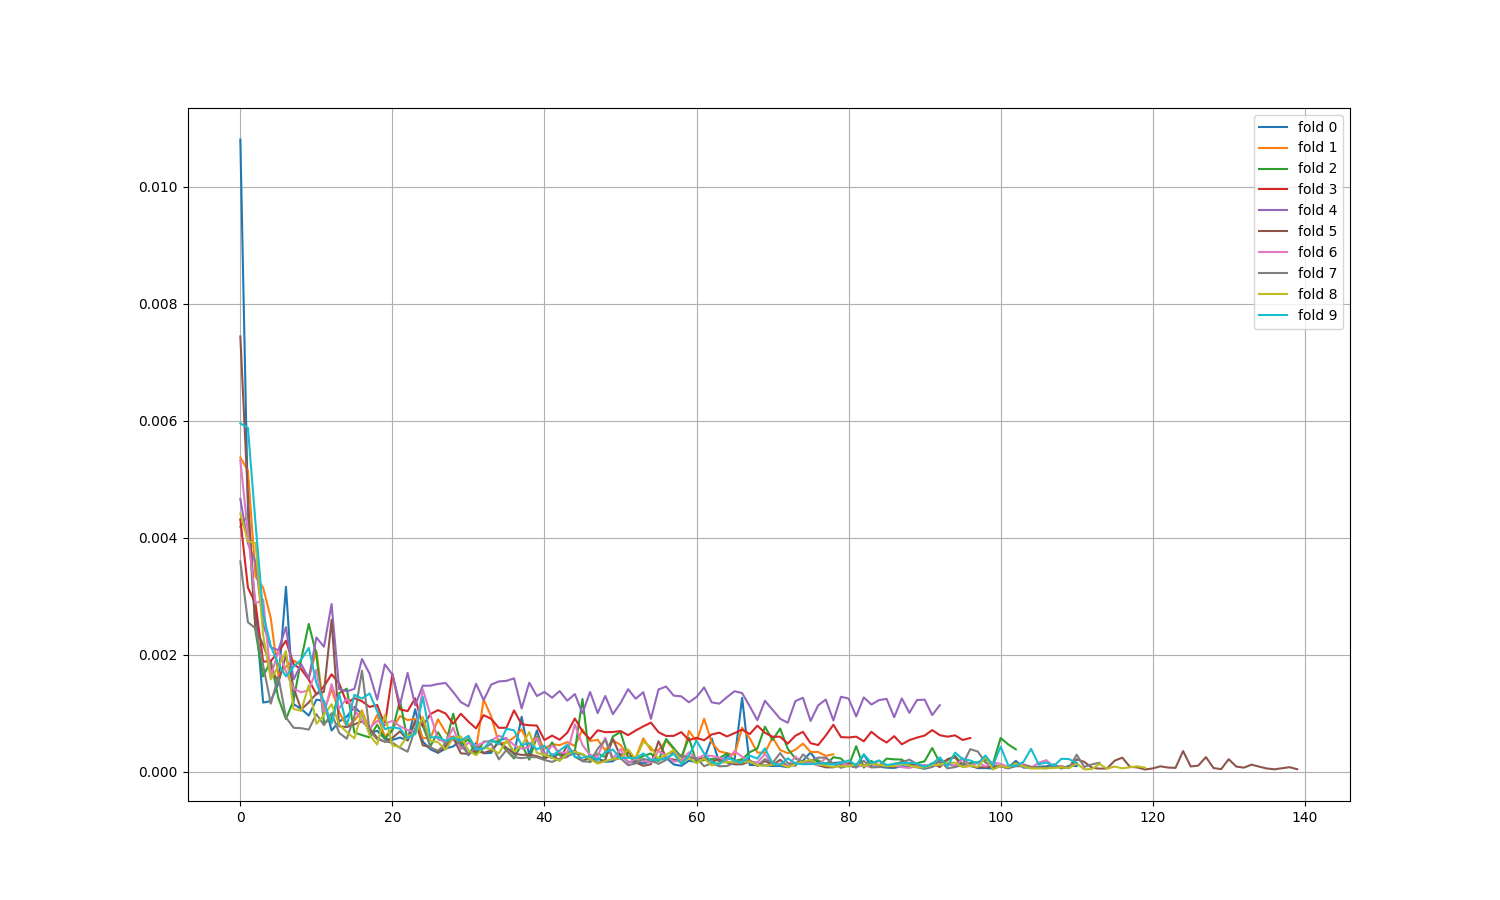
\includegraphics[width=\linewidth]{blstm-hidden-loss}
    \caption{validation loss function per fold in BLSTM with hidden layer model}
\end{figure}

\end{document}
